\chapter{Biblioteca Mathematical Components}
\label{cap:mathcomp}

Nos capítulos seguintes será usada uma série de itens disponíveis na biblioteca Mathematical Components e outros implementados com uso da biblioteca. Todavia é necessário, por parte do leitor, um conhecimento básico sobre essa biblioteca, e para isso, neste capítulo serão explicados elementos que foram considerados mais essenciais de acordo com o tema definido. Todo o conteúdo a seguir se baseia em \cite{assia_mahboubi_2022_7118596}.

Ademais, é importante ressaltar que, na apresentação dos conteúdos deste capítulo, se assume que o leitor possui um conhecimento básico sobre \textit{Coq}, e em caso contrário recomenda-se que o leitor acesse o material disponível em: \url{https://softwarefoundations.cis.upenn.edu/lf-current/index.html}

\section{Módulos}
A biblioteca Mathematical Components é divida em módulos, nos quais alguns são simplesmente a união de outros menores relacionados entre si. No site oficial da biblioteca\footnote{\url{https://math-comp.github.io/}} está disponível, além do livro utilizado como referência neste trabalho \cite{assia_mahboubi_2022_7118596}, um grafo
de tais módulos. A Figura \ref{fig:graph-mathcomp} apresenta uma parte desse grafo:

\begin{figure}[h]
    \centering
    \caption{Print de parte do grafo dos módulos da biblioteca Mathematical Components}
    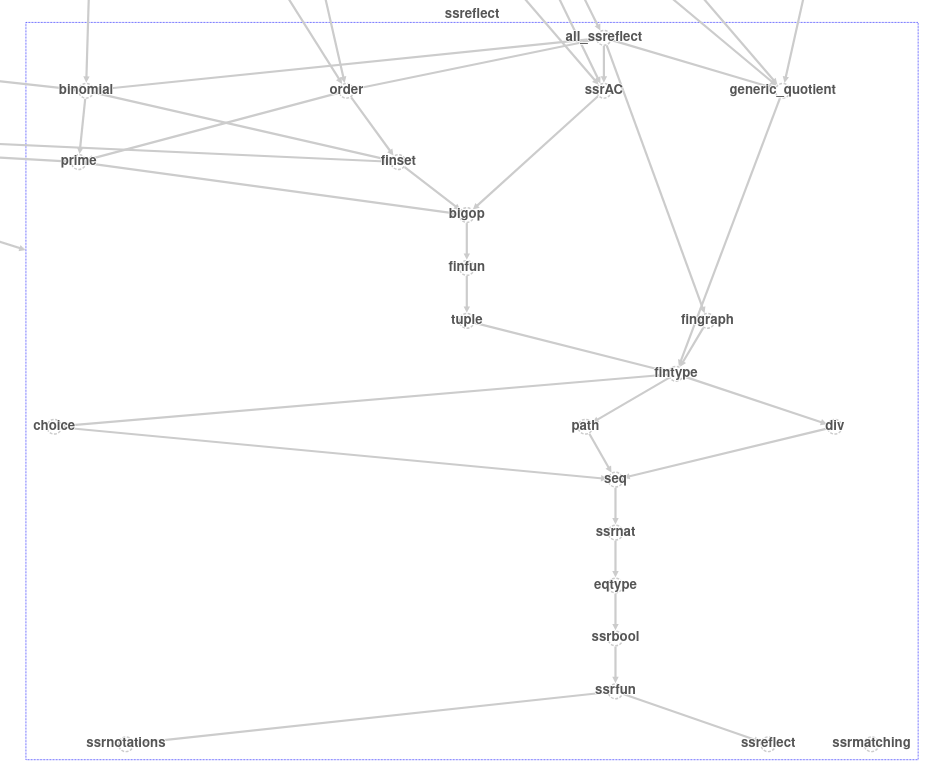
\includegraphics[width=0.6\textwidth]{Figuras/ssreflect.png}\\
    \footnotesize{Fonte:\citeauthor{grafo-ssreflect}, \citeyear{grafo-ssreflect}.
    %Acesso em: 18 de maio de 2024.
    }
    \label{fig:graph-mathcomp}
\end{figure}

% Os módulos principais para o desenvolvimento da prova sobre o algoritmo Tonelli-Shanks (com base no conteúdo de Teoria dos Números que sustenta a lógica do mesmo) são: \textit{all\_ssreflect} (que contém diversos outros módulos), \textit{ring\_quotient}, \textit{zmodp} e \textit{intdiv}.

\section{Igualdades}
Na maior parte dos teoremas das bibliotecas nativas de \textit{Coq}, usa-se uma definição indutiva de igualdade, que é por sua vez equivalente a igualdade de Leibniz (isto pode ser provado). Por sua vez, essa definição de igualdade é dada pela seguinte proposição indutiva (de acordo com a documentação \cite{coqteam2022manual}) na Figura \ref{fig:inductive-eq}:
    \begin{figure}[h]
    \centering
    \caption{Código da proposição indutiva para igualdade}
\begin{lstlisting}[language=coq,frame=single,tabsize=1]
Inductive eq (A : Type) (x : A) : A -> Prop := 
    eq_refl : eq A x x.
\end{lstlisting}
    \footnotesize{Fonte: adaptado de \citeauthor{coqteam2022manual}, \citeyear{coqteam2022manual}.
    }
    \label{fig:inductive-eq}
    \end{figure}

De maneira distinta, a biblioteca Mathematical Components, em suas definições e teoremas, utiliza com frequência predicados booleanos \cite{assia_mahboubi_2022_7118596}, que são basicamente funções cujo tipo de retorno é \lstinline[language = coq]!bool!, para então representar proposições da forma \lstinline[language = coq]$x = true$, onde \lstinline[language = coq]$x$ é uma expressão cujo retorno é do tipo \lstinline[language = coq]!bool!. Tais proposições são construídas pela função \lstinline[language = coq]$is_true$. No entanto, através do comando \lstinline[language = coq]$Coercion$ (que será explicado mais detalhadamente adiante neste documento) e por questões de legibilidade, tal função é omitida e o sistema de tipos de \textit{Coq} é capaz de inferir quando uma expressão deve ter tipo \lstinline[language = coq]$bool$ ou tipo \lstinline[language = coq]$Prop$ (e então há uma aplicação de \lstinline[language = coq]$is_true$ omitida). 

Semelhantes aos teoremas existentes para proposição comuns, estão disponíveis diversos teoremas para proposições geradas com o uso de \lstinline[language = coq]$is_true$, como por exemplo o lema \lstinline[language = coq]$contraLR$ apresentado em \cite{assia_mahboubi_2022_7118596}. Esse é uma versão da contraposição utilizando predicados booleanos (junto à função \lstinline[language = coq]$is_true$) e sua definição, conforme \cite{assia_mahboubi_2022_7118596}, é dada na Figura \ref{fig:lemma-contraLR}:
\begin{figure}[h]
    \centering
    \caption{Código do lema \coqinline[]{contraLR}}
    \begin{lstlisting}[language=coq,frame=single,tabsize=1]
Lemma contraLR (c b : bool) : (~~ c -> ~~ b) -> b -> c.
    \end{lstlisting}
    \footnotesize{Fonte: adaptado de \citeauthor{assia_mahboubi_2022_7118596}, \citeyear{assia_mahboubi_2022_7118596}.
    }
    \label{fig:lemma-contraLR}
\end{figure}
\\onde \lstinline[language = coq]$~~$ é a operação de negação definida na biblioteca Mathematical Components.

Outra informação relevante ao se tratar do conteúdo da biblioteca é o tipo \lstinline[language = coq]$eqType$: para que seja construído qualquer habitante desse tipo é necessário um elemento \lstinline[language = coq]$T$ de tipo 
\lstinline[language = coq]$Type$, uma função \lstinline[language = coq]$eq_op$ de tipo \lstinline[language = coq]$T -> T -> bool$
e um elemento \lstinline[language = coq]$eqP$ cujo tipo é um teorema relacionando a igualdade de Leibniz com \lstinline[language = coq]$T$ e \lstinline[language = coq]$eq_op$. Esse último possui, na biblioteca, uma notação de nome \lstinline[language = coq]$eq_axiom$, e sua descrição, dada em \cite{mathcomp-eqtype}, é apresentada na Figura \ref{fig:definition-eqaxiom} (onde \lstinline[language = coq]$rel T$ é equivalente ao tipo \lstinline[language = coq]$T -> T -> bool$):
%     \begin{lstlisting}[language=coq,frame=single,tabsize=1]
% Definition eq_axiom: forall (T : Type) (e : rel T), forall x x0 : T, 
%     reflect (x = x0) (e x x0)
%     \end{lstlisting}
\begin{figure}[ht]
    \centering
    \caption{Código da definição \coqinline[]{eq_axiom}}
    \begin{lstlisting}[language=coq,frame=single,tabsize=1]
Definition eq_axiom T (e : rel T) := forall x y, reflect (x = y) (e x y).
    \end{lstlisting}
    \footnotesize{Fonte: adaptado de \citeauthor{mathcomp-eqtype}, \citeyear{mathcomp-eqtype}.
    }
    \label{fig:definition-eqaxiom}
\end{figure}
\\
% \\onde \lstinline[language = coq]$rel T$ é equivalente ao tipo \lstinline[language = coq]$T -> T -> bool$.

Portanto, para que um tipo \lstinline[language = coq]$A$
pertença ao primeiro campo mencionado, é necessário que se tenha uma prova da proposição \lstinline[language = coq]$eq_axiom A$, isto é, 
a definição \lstinline[language = coq]$eq_axiom$ com 
\lstinline[language = coq]$T$ igual a \lstinline[language = coq]$A$.

% Tal teorema indica que a igualdade sobre \lstinline[language = coq]$A$
% é decidível, o que fica claro pelo seguinte lema:
%     \begin{lstlisting}[language=coq,frame=single,tabsize=1]
% Lemma decP: forall (P : Prop) (b : bool), reflect P b -> decidable P
%     \end{lstlisting}

A utilização de um tipo como \lstinline[language = coq]$eqType$ facilita que se provem teoremas genéricos, no sentido de que servem para diferentes tipos (pertencentes a \lstinline[language = coq]$Type$) desde que estes possuam uma relação de equivalência decidível. Existem outros tipos semelhantes a \lstinline[language = coq]$eqType$, no sentido de que servem como interfaces. Em grande parte, esses são implementados por meio do açúcar sintático \lstinline[language = coq]$Record$, qual será explicado na sessão seguinte.

\section{Structures e Records} 
\label{section:structs-e-records}

\lstinline[language = coq]$Structure$ e \lstinline[language = coq]$Record$ são comandos sinônimos para geração de tipos indutivos que possuem somente um construtor e cujo os campos são dependentemente tipados, isto é, o tipo de cada campo pode depender dos valores de campos anteriores, assim como nas definições indutivas \cite{assia_mahboubi_2022_7118596}. A vantagem do uso desses comandos é que por meio desses são geradas automaticamente funções para extrair valores dos argumentos do construtor do tipo declarado.

Esses comandos são frequentemente utilizados na biblioteca Mathematical Components para definir interfaces (como o \lstinline[language = coq]$eqType$) e subtipos (ex.: tipo em que os habitantes são todos os números naturais menores que $8$). Para melhor entendimento do leitor, tem-se a seguir um exemplo semelhante ao tipo \lstinline[language = coq]$eqType$ definido em \cite{assia_mahboubi_2022_7118596} porém que contém também o campo \coqinline[]{axiom}:
    % \begin{figure}[h]
    % \centering
    % \caption{Código do lema \coqinline[]{contraLR}}
\begin{lstlisting}[language=coq,frame=single,tabsize=1]
Record eqType : Type := Pack {
    sort : Type;
    eq_op : sort -> sort -> bool;
    axiom : eq_axiom op
}.
\end{lstlisting}
    % \footnotesize{Fonte: o autor (2024).}
    % \label{fig:record-eqType}
    % \end{figure}
% \\
Como explicado acima, essa declaração é equivalente a se fazer as seguintes declarações:
    \begin{lstlisting}[language=coq,frame=single,tabsize=1]
Inductive eqType : Type :=
    | Pack (sort : Type) (op : sort -> sort -> bool) (axiom : eq_axiom eq_op).
    
Definition sort (e : eqType) : Type :=
    match e with
    | Pack t _ _ => t
    end.
Definition eq_op (e : eqType) : (sort e -> sort e -> bool) :=
    match e with
    | Pack _ f _ => f
    end.
Definition axiom (e : eqType) : (eq_axiom (eq_op e)) :=
    | Pack _ _ a => a
    end.
    \end{lstlisting}
Observe que o uso de tipos dependentes ocorre nos campos \lstinline[language = coq]{eq_op} e \lstinline[language = coq]{axiom}. No primeiro, o tipo do campo depende do valor do campo \lstinline[language = coq]{sort} e no segundo o tipo do campo depende do valor do campo \lstinline[language = coq]{eq_op} e portanto também do campo \lstinline[language = coq]{sort}.

\subsection{Comando Canonical} De modo semelhante ao apresentado em \cite{assia_mahboubi_2022_7118596}, para instanciar um habitante de \lstinline[language = coq]$eqType$ com campo \lstinline[language = coq]$sort$ igual a \lstinline[language = coq]$nat$, deve-se provar o seguinte teorema:
    \begin{lstlisting}[language=coq,frame=single,tabsize=1]
Theorem axiom_nat: eq_axiom eqn.
    \end{lstlisting}
onde \lstinline[language = coq]$eqn$ é uma operação de comparação booleana entre números naturais.
Tendo esta prova, como feito em \cite{assia_mahboubi_2022_7118596}, podemos instanciar tal habitante
da seguinte forma:
    \begin{lstlisting}[language=coq,frame=single,tabsize=1]
Definition natEqtype := Pack nat eqn axiom_nat.
    \end{lstlisting}
Note que, agora, pode-se comparar dois números naturais da seguinte maneira:
    \begin{lstlisting}[language=coq,frame=single,tabsize=1]
Compute (@eq_op natEqType 2 2).
    \end{lstlisting}
o que nesse caso equivale a:
    \begin{lstlisting}[language=coq,frame=single,tabsize=1]
Compute (eqn 2 2).
    \end{lstlisting}

Entretanto, o objetivo de criar o tipo \lstinline[language = coq]$eqType$ não é estabelecer essa possibilidade de computação para relações de comparação, mas sim construir definições, funções e provas genéricas para todos os tipos que pertencem ao campo \lstinline[language = coq]$sort$ de algum habitante de \lstinline[language = coq]$eqType$ e estabelecer \textit{overloading} de notações. Para exemplo de como alcançar este último objetivo, em \cite{assia_mahboubi_2022_7118596} se define uma notação da seguinte forma exposta na Figura \ref{fig:notation-eqop}:
\begin{figure}[ht]
    \centering
    \caption{Código da notação ``\coqinline[]{==}''}
\begin{lstlisting}[language=coq,frame=single,tabsize=1]
Notation "x == y" := (@eq_op _ x y).
\end{lstlisting}
    \footnotesize{Fonte: adaptado de \citeauthor{assia_mahboubi_2022_7118596}, \citeyear{assia_mahboubi_2022_7118596}.
    }
    \label{fig:notation-eqop}
\end{figure}
%     \begin{lstlisting}[language=coq,frame=single,tabsize=1]
% Notation "x == y" := (@eq_op _ x y).
%     \end{lstlisting}
\\

\noindent porém havendo apenas esta definição, caso executado o comando \lstinline[language = coq]$Check (3 == 2)$ tem-se um falha. Ao se executar:
    \begin{lstlisting}[language=coq,frame=single,tabsize=1]
Fail Check (3 == 11).
    \end{lstlisting}
% Fail Check (3 == 2).
a seguinte mensagem é apresentada:
    \begin{lstlisting}[language=coq-error,frame=single,tabsize=1]
The command has indeed failed with message:
The term "3" has type "nat" while it is 
expected to have type "sort ?e"
    \end{lstlisting}
Isto ocorre pois o \textit{Coq} não é capaz de inferir o argumento implícito\footnote{Note que o comando \lstinline[language = coq]$Fail Check (3 == 2)$ é equivalente a \lstinline[language = coq]$Fail Check (@eq_op _ 3 2)$.}  (\lstinline[language = coq]$_$).

Note que é mencionada uma variável \lstinline[language = coq]$?e$. Essa representa um elemento a ser inferido de modo que o tipo \lstinline[language = coq]$sort ?e$ seja igual ao tipo \lstinline[language = coq]$nat$. Como exposto em \cite{10.1007/978-3-642-39634-2_5} o algoritmo de inferência do \textit{Coq} não é capaz de descobrir o valor de tal variável por meio das regras de inferência que possui. Para resolver este problema, conforme \cite{assia_mahboubi_2022_7118596}, 
o \textit{Coq} permite que se adicione regras de inferência de tipo por meio do comando \lstinline[language = coq]$Canonical$ (que recebe um construtor de algum \lstinline[language = coq]$Record$ ou \lstinline[language = coq]$Structure$ aplicado aos seus argumentos). Assim, resolver esse problema é possível por meio do seguinte código:
    \begin{lstlisting}[language=coq,frame=single,tabsize=1]
Canonical natEqType.
    \end{lstlisting}
Com isto, de maneira semelhante ao exemplo exposto em \cite{10.1007/978-3-642-39634-2_5}, é adicionada a seguinte regra de inferência ao algoritmo presente em \textit{Coq}:

\begin{equation*}
        \inferrule 
        {
        \text{\lstinline[language = coq]!nat!} \sim 
        \text{\lstinline[language = coq]!sort natEqType!} 
        \\
        \; \text{\lstinline[language = coq]!?!} \text{\lstinline[language = coq]!e!} \; \sim
        \text{\lstinline[language = coq]!natEqType!} 
        }
        {\text{\lstinline[language = coq]!nat!} \sim \text{\lstinline[language = coq]!sort ?e!}}   
\end{equation*}
em que a notação $\sim$ representa uma chamada do algoritmo de unificação \cite{10.1007/978-3-642-39634-2_5} (que é o nome dado ao algoritmo de comparação de tipos chamado nas rotinas de inferência de tipos). Neste momento o leitor pode se perguntar como tal regra de inferência leva o algoritmo a chegar em um resultado final, e a resposta de acordo \cite{10.1007/978-3-642-39634-2_5} está em na existência de outras regras de inferência, como \textit{eq} e \textit{assign}:
\begin{equation*}
    \inferrule
    { }
    {
        \text{\lstinline[language = coq]!t!} \sim \text{\lstinline[language = coq]!t!}
    } \textit{eq}
    \hspace{20mm} % \text{&&}
    \inferrule
    { }
    {
        \text{\lstinline[language = coq]!?!\lstinline[language = coq]!x!} \sim \text{\lstinline[language = coq]!t!}
    } \textit{assign}
\end{equation*}
Retornando ao comando \lstinline[language = coq]$Check$, se agora esse for executado da mesma maneira feita anteriormente (porém sem o \lstinline[language = coq]$Fail$):
    \begin{lstlisting}[language = coq,frame=single,tabsize=1]
Check (3 == 11).
    \end{lstlisting}
tem-se o seguinte resultado:
    \begin{lstlisting}[language = coq-error,frame=single,tabsize=1]
3 == 11
    : bool
    \end{lstlisting}

Como mencionado previamente o tipo \lstinline[language = coq]$eqType$ serve para diversas generalizações. Para exemplo disso, adiante se apresenta a definição de uma comparação entre valores do tipo \lstinline[language = coq]$option$. Antes desse exemplo, vale aqui relembrar o leitor da definição deste tipo:
\begin{figure}[h]
    \centering
    \caption{Código do lema \coqinline[]{contraLR}}
    \begin{lstlisting}[language = coq,frame=single,tabsize=1]
Inductive option (A : Type) : Type :=
    | None : option A
    | Some : A -> option A.
    \end{lstlisting}
\footnotesize{Fonte: adaptado de \citeauthor{coqteam2022manual}, \citeyear{coqteam2022manual}.}
    \label{fig:inductive-option}
    \end{figure}
A função de comparação a ser declarada irá considerar que o argumento \lstinline[language = coq]$A$ pertence ao campo \lstinline[language = coq]$sort$ de algum habitante de \lstinline[language = coq]$eqType$. Tem-se então a definição dessa função:
    \begin{lstlisting}[language = coq,frame=single,tabsize=1]
Definition cmp_option (e : eqType) (o1 o2 : option (sort e)) :=
    match o1, o2 with
    | Some e1, Some e2 => op e e1 e2
    | None, Some _ => false
    | Some _, None => false
    | None, None => true
    end.
    \end{lstlisting}
Agora, para criar um habitante de \lstinline[language = coq]$eqType$ para todo tipo da forma \lstinline[language = coq]$option A$ (note que para todo \lstinline[language = coq]$A$ diferente tem-se um tipo diferente) em que o tipo \lstinline[language = coq]$A$ segue o que foi considerado na função, deve-se provar o seguinte teorema:
    \begin{lstlisting}[language = coq,frame=single,tabsize=1]
Theorem axiom_option: 
    forall e : eqType, eq_axiom (cmp_option e).
    \end{lstlisting}
que para facilidade de entendimento do leitor, pode ser escrito como:
    \begin{lstlisting}[language = coq,frame=single,tabsize=1]
Theorem axiom_option: 
    forall e : eqType, forall x y : option (sort e), reflect (x = y) (@cmp_option e x y).
    \end{lstlisting}
Com esta prova pode-se construir a seguinte definição:
    \begin{lstlisting}[language = coq,frame=single,tabsize=1]
Definition optionEqType (e : eqType) := 
    Pack (option (sort e)) (cmp_option e) (axiom_option e).
    \end{lstlisting}
Visto que ainda não foi executado o comando \lstinline[language = coq]$Canonical$ com esta definição, se executado o comando \lstinline[language = coq]$Check (Some 1 == Some 11)$, esse irá falhar, logo, ao se executar:
    \begin{lstlisting}[language = coq,frame=single,tabsize=1]
Fail Check (Some 1 == Some 11).
    \end{lstlisting}
É apresentada a seguinte mensagem:
    \begin{lstlisting}[language = coq-error,frame=single,tabsize=1]
The command has indeed failed with message:
The term "Some 1" has type "option nat" 
while it is expected to have type "sort ?e".
    \end{lstlisting}
Semelhante ao que foi feito anteriormente, para resolver este problema deve-se executar: 
    \begin{lstlisting}[language = coq,frame=single,tabsize=1]
Canonical optionEqType.
    \end{lstlisting}
e com isso se adiciona a seguinte regra de inferência:
% Semelhante ao que foi feito anteriormente, para resolver este problema deve-se executar: 
%     \begin{lstlisting}[language = coq,frame=single,tabsize=1]
% Canonical optionEqType.
%     \end{lstlisting}
% e com isso se adiciona a seguinte regra de inferência:
\begin{equation*}
    \inferrule
    {
    \text{\lstinline[language = coq]!t!} \sim 
    \text{\lstinline[language = coq]!sort ?x!} 
    \\ 
    \text{\lstinline[language = coq]!?!\lstinline[language = coq]!e!} \sim
    \text{\lstinline[language = coq]!optionEqType ?x!} 
    }
    {
        \text{\lstinline[language = coq]!option t!} \sim \text{\lstinline[language = coq]!sort ?e!}
    }   
\end{equation*}
Assim note que no problema de inferência acima, ocorre a seguinte (sub)sequência de aplicação de regras de inferência para se determinar o valor de \lstinline[language = coq]$?e$:
\begin{equation*}
    \inferrule []
    {
        \inferrule []
        {
        \text{\lstinline[language = coq]!nat!} \sim 
        \text{\lstinline[language = coq]!sort natEqType!} 
        \\ 
        \text{\lstinline[language = coq]!?!\lstinline[language = coq]!x!} \sim
        \text{\lstinline[language = coq]!natEqType!} 
        }
        {\text{\lstinline[language = coq]!nat!} \sim \text{\lstinline[language = coq]!sort ?x!}} 
        % \lstinline[language = coq]!nat! \sim 
        % \lstinline[language = coq]!sort ?x! 
        \\ 
        \\
        \text{\lstinline[language = coq]!?!\lstinline[language = coq]!e!} \sim
        \text{\lstinline[language = coq]!optionEqType ?x!} 
    }
    {\text{\lstinline[language = coq]!option nat!} \sim \text{\lstinline[language = coq]!sort ?e!}}   
\end{equation*}
Agora, com o comando:
    \begin{lstlisting}[language = coq,frame=single,tabsize=1]
Check (Some 1 == Some 11).
    \end{lstlisting}
tem-se a mensagem:
    \begin{lstlisting}[language = coq-error,frame=single,tabsize=1]
Some 1 == Some 11
    : bool
    \end{lstlisting}

\subsection{Comando Coercion} \label{subsection:coercion}

Em provas manuais costuma-se utilizar notações iguais para operações sobre diferentes tipos. Como exemplo, há o uso do símbolo $+$ para operação de soma sobre os conjuntos númericos $\mathbb{N}$, $\mathbb{Z}$, $\mathbb{Q}$, $\mathbb{R}$ , como operador lógico \textit{ou} e também como operação binária qualquer que forma um monoide genérico. Nessa aplicação cotidiana de \textit{overloading} de notações, as informações sobre tipos são inferidas pelo cérebro humano conforme o contexto em que se encontram \cite{10.1007/978-3-642-39634-2_5}. 
Tomando isso em consideração e tendo em mente o conteúdo abordado na subseção anterior, pode-se dizer que o comando \lstinline[language = coq]$Canonical$ auxilia os usuários, tornando a escrita em \textit{Coq} mais semelhante a que se faz manualmente.

Outro mecanismo relacionado a tipos em \textit{Coq}, e que de certa forma serve para esse mesmo propósito, é provido pelo comando \lstinline[language = coq]$Coercion$. Como motivação para o uso deste, suponha a declaração em \textit{Coq} de um tipo que contenha todos os números naturais múltiplos de um número $n$. Utilizando \lstinline[language = coq]$Record$, temos então: 
    \begin{lstlisting}[language = coq,frame=single,tabsize=1]
Record multiple (n : nat) : Type := Build
{       
    x : nat;
    axiom : (n %| x)        
}.
    \end{lstlisting}
Observe que para construir um habitante deste tipo é dado um elemento \lstinline[language = coq]$n$ de tipo \lstinline[language = coq]$nat$ e é necessário um elemento \lstinline[language = coq]$x$ de mesmo tipo, e além disso, uma prova\footnote{Há de maneira implícita a aplicação da função \lstinline[language = coq]$is_true$ no tipo do campo \lstinline[language = coq]$axiom$, portanto o que foi declarado como tipo deste campo, isto é, \lstinline[language = coq]$n \%| x$, é equivalente a \lstinline[language = coq]$n \%| x = true$.} de que \lstinline[language = coq]$x$ é divisível por \lstinline[language = coq]$n$.
Agora, com tal declaração, visto que o objetivo da mesma é representar qualquer conjunto de números divisíveis por um determinado natural $n$, o usuário de \textit{Coq} provavelmente desejará que se possa escrever algo como:
    \begin{lstlisting}[language = coq,frame=single,tabsize=1]
forall (n : nat) (a : multiple n), a + 0 = a.
    \end{lstlisting}
sem que o uso da operação de adição leve a um erro pela razão dessa possuir tipo \lstinline[language = coq]$nat -> nat -> nat$ enquanto o argumento \lstinline[language = coq]$a$ tem tipo \lstinline[language = coq]$multiple n$, quando a intenção do usuário é de que este último represente um número natural. Se for utilizado o comando \lstinline[language = coq]$Check$ na proposição acima:
    \begin{lstlisting}[language = coq,frame=single,tabsize=1]
Fail Check (forall (n : nat) (a : multiple n), a + 0 = a).
    \end{lstlisting}
tem-se a mensagem:
    \begin{lstlisting}[language = coq-error,frame=single,tabsize=1]
The command has indeed failed with message:
In environment
n : nat
a : multiple n
The term "a" has type "multiple n" while it is
expected to have type "nat".
    \end{lstlisting}
Buscando solucionar este tipo de problema, sem que tenha que se escrever:
    \begin{lstlisting}[language = coq,frame=single,tabsize=1]
forall (n : nat) (a : multiple n), (x n a) + 0 = (x n a).
    \end{lstlisting}
o que por sua vez não geraria erro algum pois \lstinline[language = coq]$(x n a)$ tem tipo \lstinline[language = coq]$nat$\footnote{Lembre-se que \lstinline[language = coq]$x$, no contexto externo a declaração do seu respectivo \lstinline[language = coq]$Record$, é uma função que extrai o campo \lstinline[language = coq]$x$ de um elemento do tipo \lstinline[language = coq]$multiple n$ (para qualquer \lstinline[language = coq]$n$) e não o valor do campo em si. Portanto a seguinte definção poderia ser dada simplesmente como \lstinline[language = coq]$x$.}, defini-se uma função que retira o campo \lstinline[language = coq]$x$ de um elemento como \lstinline[language = coq]$a$:
    \begin{lstlisting}[language = coq,frame=single,tabsize=1]
Definition multiple_nat (n : nat) (e : multiple n) : nat :=
    let t := (x n e) in t.
    \end{lstlisting}
e agora, para que o \textit{Coq} aplique esta função de maneira implícita, de modo a evitar erros de tipo, usa-se o comando \lstinline[language = coq]$Coercion$ da seguinte maneira:
    \begin{lstlisting}[language = coq,frame=single,tabsize=1]
Coercion multiple_nat : multiple >-> nat.
    \end{lstlisting}
Agora, realizando o comando \lstinline[language = coq]$Check$ como anteriormente:
    \begin{lstlisting}[language = coq,frame=single,tabsize=1]
Check (forall n (a : multiple n), a + 0 = 0).
    \end{lstlisting}
é gerada a mensagem:
    \begin{lstlisting}[language = coq-error,frame=single,tabsize=1]
forall (n : nat) (a : multiple n), a + 0 = 0
    : Prop
    \end{lstlisting}

\subsection{Exemplo de Implementação de Grupos}
\label{sub:grupos}

Um uso semelhante do mecanismo \textit{coercion}, junto ao \textit{canonical}, pode ser proposto com um tipo que representa grupos. Um grupo é uma estrutura algébrica dada por $(G, \otimes)$ onde $G$ é um conjunto e:
\begin{enumerate}
    \item $\otimes$ é uma operação binária sobre $G$, isto é, $\otimes$ é uma função tal que $\otimes : (G \times G) \rightarrow G$.
    \item $\otimes$ é associativa, ou seja, $\forall a, b \in G, (a \otimes b) \otimes c = a \otimes (b \otimes c)$.
    \item Existe um elemento neutro $e$, o que significa: $\exists e \in G (\forall a \in G, e \otimes a = a \otimes e = a)$. 
    \item Para todo elemento em $G$ existe um elemento inverso, isto é, \\
    $\forall x \in G (\exists \;\overline{x} \in G, x \;\otimes\; \overline{x} = \overline{x} \;\otimes\; x = e)$
\end{enumerate}
Em \textit{Coq} um grupo pode ser representado pelo seguinte \lstinline[language = coq]$Record$:
    \begin{lstlisting}[language = coq,frame=single,tabsize=1]
Record Group : Type := group 
{
    sort :> Type;
    bin_op : sort -> sort -> sort;
    associative_axiom : associative bin_op;
    e : sort;
    neutral_left : left_id e bin_op;
    neutral_right : right_id e bin_op;
    inverse_left : \forall x : sort, \exists y : sort, bin_op y x = e; 
    inverse_right : \forall x : sort, \exists y : sort, bin_op x y = e 
}.
    \end{lstlisting}
Observe que, diferente dos exemplos anteriores, o campo \lstinline[language = coq]$sort$ é seguido de \lstinline[language = coq]$:>$. Esse operador além de atribuir o tipo de \lstinline[language = coq]$sort$ como \lstinline[language = coq]$Type$
define a função \lstinline[language = coq]$sort$ como uma \textit{coercion} para todo habitante do tipo \lstinline[language = coq]$Group$. Assim, suponha a definição do seguinte habitante:
    \begin{lstlisting}[language = coq,frame=single,tabsize=1]
Definition int_group := 
    Group int addz addzA 0 add0z addz0 inverse_left_int inverse_right_int.
    \end{lstlisting}
Esse habitante tem como campo \lstinline[language = coq]$sort$ o tipo \lstinline[language = coq]$int$ (que representa os números inteiros) e devido a \textit{coercion}, se for feita uma declaração com uma variável de tipo \lstinline[language = coq]$int_group$ em que se aplica uma função de tipo \lstinline[language = coq]$int -> int$ sobre esta variável, o \textit{Coq} irá automaticamente tratar a variável como tendo tipo \lstinline[language = coq]$int$ (ou mais especificamente, irá tratá-la como se fosse o valor de seu campo \lstinline[language = coq]$sort$, aplicando de maneira implícita a função \lstinline[language = coq]$sort$ sobre a mesma).

Para fins de demonstrar uma implentação completa de grupos em \textit{Coq}, define-se agora uma notação para as operações binárias e uma para os elementos neutros que formam grupos quaisquer, da seguinte forma:
    \begin{lstlisting}[language = coq,frame=single,tabsize=1]
Notation "x \otimes y" := (@bin_op _ x y) (at level 10).
Notation "0" := (@e _).
    \end{lstlisting}
Usa-se então o comando \lstinline[language = coq]$Canonical$ para que o \textit{Coq} seja capaz de inferir os argumentos implícitos presentes nas descrições destas notações (para o caso de \lstinline[language = coq]$x$ e  \lstinline[language = coq]$y$ possuirem tipo  \lstinline[language = coq]$int$):
    \begin{lstlisting}[language = coq,frame=single,tabsize=1]
Canonical int_group.
    \end{lstlisting}
Com este conjunto de configurações passa a ser mais fácil a escrita e leitura de declarações relacionadas a grupos. Assim, torna-se então possível a formalização compacta de teoremas genéricos sobre quaisquer tipos presentes no campo \lstinline[language = coq]$sort$ de algum habitante de \lstinline[language = coq]$group$. Como exemplo, tem-se o seguinte teorema e sua respectiva prova:
    \begin{lstlisting}[language = coq,frame=single,tabsize=1, escapechar=@]
Theorem exemplo_sobre_grupos: 
    \forall G : group, \forall a b : G, (a \otimes b) \otimes 0 = (a \otimes 0) \otimes b.
Proof.
    intros.
    rewrite neutral_right. 
    rewrite neutral_right.
    reflexivity. 
Qed.
    \end{lstlisting}
onde no lugar de \coqinline[]{neutral_right} seria equivalente utilizar \coqinline[]{(neutral_right _)} ou também \coqinline[]{(neutral_right G)}. 

Como este teorema serve para qualquer grupo \lstinline[language = coq]$G$, esse pode então ser usado na seguinte prova:
    \begin{lstlisting}[language = coq,frame=single,tabsize=1]
Theorem exemplo_sobre_int:
    \forall a b : int, (a + b) + 0 = (a + 0) + b.
Proof.
    apply exemplo_sobre_grupos.
Qed.
    \end{lstlisting}
Tal prova exemplifica como o uso dos mecanismos em \textit{Coq}, que foram apresentados neste capítulo, podem ser utilizados para que seja mais fácil trabalhar com um vasta quantidade de tipos que apresentam propriedades em comum (como é o caso dos grupos).

\subsection{Mecanismo para Hierarquias entre Estruturas Algébricas}

Para organizar estruturas algébricas semelhantes a apresentada na Subseção \ref{sub:grupos}, a biblioteca Mathematical Components utiliza uma linguagem chamada $\mathcal{HB}$. Esta é disponibilizada em \textit{Coq} por meio do \textit{addon} \coqinline!hierarchy-builder! e a motivação por trás de seu uso é facilitar aos usuários a criação, manutenção e padronização destas estruturas. Caso o leitor deseje um aprofundamento nestes assuntos recomenda-se a publicação e o vídeo nos quais esta subseção é baseada que são eles \cite{cohen:hal-02478907} e \cite{youtuCohen} respectivamente. Se faz esta recomendação pois o sistema por trás do gerenciamento de tais estruturas não faz parte do escopo deste trabalho. Nesta subseção se busca apenas mostrar como o usuário pode pesquisar propriedades provadas sobre um determinado tipo por meio de estruturas com a qual o tipo está ``equipado'', expressão cujo significado será explicado adiante.

% Diversas estruturas como as algébricas, que guardam predicados sobre tipos, são utilizadas na biblioteca Mathematical, e suas declarações seguem um padrão chamado de 

Ao se utilizar a biblioteca Mathematical Components pela primeira vez o usuário tende a necessitar corriqueiramente da ferramenta de busca de teoremas, lemas e definições. Isto tende acontecer pois em geral o usuário precisa aprender os nomes (e padrões destes) utilizados na biblioteca e como são implementados. Como exemplo, suponha que queira-se rescrever uma expressão com números naturais utilizando a propriedade de comutatividade. Para isso, o usuário pode utilizar o comando \coqinline|Search| junto a um padrão para pesquisa:
    \begin{lstlisting}[language=coq,frame=single,tabsize=1]
Search (_ + _).
    \end{lstlisting}
ou, caso queira fazer uma pesquisa mais precisa dentro do escopo \coqinline|nat_scope|, pode usar:
    \begin{lstlisting}[language=coq,frame=single,tabsize=1]
Search (_ + _)%N.
    \end{lstlisting}
Esse último comando traz a seguinte mensagem:
    \begin{lstlisting}[language=coq-error,frame=single,tabsize=1, escapechar=@, escapechar=@, numbers=left]
rshift: forall (m : nat) [n : nat], 'I_n -> 'I_(m + n)
lshift: forall [m : nat] (n : nat), 'I_m -> 'I_(m + n)
addnn: forall n : nat, n + n = n.*2
leq_addl: forall m n : nat, n <= m + n
leq_addr: forall m n : nat, n <= n + m      @ \Suppressnumber @
    (*... continua...*)                     @ \Reactivatenumber @
    \end{lstlisting}
No entanto, nesta lista, o usuário provavelmente não encontrará o lema que necessita, que nesse caso é \coqinline|addnC|. Isto ocorre pois o enunciado desse lema não apresenta a notação \coqinline|+|. Entretanto, fazendo a seguinte pesquisa:
    \begin{lstlisting}[language=coq,frame=single,tabsize=1]
Search commutative.
    \end{lstlisting}
onde \coqinline|commutative| é uma \textit{definition},
o lema aparece logo na linha \ref{coqlema:addn} da mensagem impressa: 
    \begin{lstlisting}[language=coq-error,frame=single,tabsize=1, escapechar=@, numbers=left]
intZmod.addzC: commutative intZmod.addz
mulnC: commutative muln
intRing.mulzC: commutative intRing.mulz
addnC: commutative addn     @ \label{coqlema:addn} @
maxnC: commutative maxn     @ \Suppressnumber @
    (*... continua...*)     @ \Reactivatenumber @
    \end{lstlisting}
Portanto o lema \coqinline|addnC| tem a seguinte definição:
    \begin{lstlisting}[language=coq,frame=single,tabsize=1]
Lemma addnC : commutative addn.
    \end{lstlisting}
Agora, supõe-se a mesma situação envolvendo números inteiros. Nesse caso, a notação \coqinline|+| aparecerá com escopo delimitado por \coqinline|%R| ou dentro do escopo \coqinline|ring_scope| ao qual \coqinline|%R| é um delimitador. A exemplo, fora de tal escopo um comando como \coqinline|Check (1%Z + 1%Z)| irá falhar, e portanto ao se executar:
    \begin{lstlisting}[language=coq,frame=single,tabsize=1]
Fail Check (1%Z + 1%Z).
    \end{lstlisting}
é apresentada a seguinte mensagem:
    \begin{lstlisting}[language=coq-error,frame=single,tabsize=1]
The command has indeed failed with message:
The term "1%Z" has type "int" while it is expected to have type "nat".
    \end{lstlisting}
enquanto o comando \coqinline|Check (1%Z + 1%Z)%R| é executado com sucesso. 

É provável então que não seja tão simples para o mesmo usuário encontrar o lema desejado, pois nesse caso, apesar da existência do lema \lstinline[language = coq]!addzC! com definição:
    \begin{lstlisting}[language=coq,frame=single,tabsize=1]
Lemma addzC : commutative addz.
    \end{lstlisting}
% pelo fato da notação \lstinline[language = coq]!+! não ser definida para a operação \lstinline[language = coq]!addz! (operação de soma entre inteiros), mesmo considerando o escopo \coqinline|ring_scope| não se pode utilizar tal lema para reescrita em uma expressão com a notação \lstinline[language = coq]!+!.
mesmo considerando o escopo \coqinline|ring_scope| não se pode utilizar tal lema para reescrita em uma expressão com a notação \lstinline[language = coq]!+!, isto pelo fato da notação \lstinline[language = coq]!+! não se referir a operação \lstinline[language = coq]!addz! a qual o lema trata. Ao invés disso, a notação mencionada se refere a operação \coqinline[]{GRing.add}, como será mosrado a seguir.

As definições de notações com utilização de um caracter como \lstinline[language = coq]!+! podem ser listadas por meio do comando \lstinline[language = coq]!Locate!, como feito a seguir:
    \begin{lstlisting}[language=coq,frame=single,tabsize=1]
Locate "+". 
    \end{lstlisting}
em que é impressa a mensagem:
    \begin{lstlisting}[language=coq-error,frame=single,tabsize=1]
Notation "{ A } + { B }" := (sumbool A B) : type_scope (default interpretation)
Notation "A + { B }" := (sumor A B) : type_scope (default interpretation)
Notation "m + n" := (Nat.add m n) : coq_nat_scope
Notation "A + B" := (addsmx.body A B) : matrix_set_scope
Notation "m + n" := (addn_rec m n) : nat_rec_scope
Notation "m + n" := (addn m n) : nat_scope (default interpretation)
Notation "x + y" := (addq x y) : rat_scope
Notation "x + y" := (GRing.add x y) : ring_scope
Notation "x + y" := (GRing.Add x y) : term_scope
Notation "x + y" := (sum x y) : type_scope
Notation "U + V" := (addv U V) : vspace_scope
    \end{lstlisting}
Pode, por esta mensagem, se verificar que a notação serve para a função \coqinline|addn| tanto no escopo \coqinline|nat_scope| quanto como interpretação padrão (\textit{default interpretation}). Também pode-se notar que a notação serve para a função \coqinline|GRing.add| (do módulo \coqinline|GRing|) no escopo \coqinline|ring_scope|, mas em nenhum momento a função \coqinline|addz| é mencionada. Verificando-se então o tipo de \coqinline|GRing.add| tem-se:
    \begin{lstlisting}[language=coq,frame=single,tabsize=1]
Print GRing.add.
    \end{lstlisting}
que gera a mensagem:
    \begin{lstlisting}[language=coq-error,frame=single,tabsize=1]
GRing.add =
fun (s : nmodType) (H : s) => [eta GRing.isNmodule.add (GRing.Nmodule.class s) H]
     : forall s : nmodType, s -> s -> s

Arguments GRing.add {s} (_ _)%ring_scope
    \end{lstlisting}
Por esta mensagem temos que \coqinline{GRing.add} tem tipo \coqinline[]{forall s : nmodType, s -> s -> s}, no entanto note que a expressão \coqinline[]{GRing.add 1%Z 1%Z} é válida (isso pode ser feito com o comando \coqinline[]{Check} ou \coqinline[]{Compute}). Isto pode parecer estranho mesmo com a possibilidade de uso do mecanismo \textit{canonical}, pois se esperava que \coqinline{GRing.add} recebesse um elemento de tipo \coqinline[]{nmodType} e retorna-se uma operação sobre o campo \coqinline[]{sort} da \textit{structure} \coqinline[]{nmodType}. Todavia, se usarmos antes do comando \coqinline[]{Print GRing.add} o comando:
    \begin{lstlisting}[language=coq,frame=single,tabsize=1]
Set Printing Coercions.
    \end{lstlisting}
a mensagem impressa pelo comando \coqinline[]{Print GRing.add} será:
    \begin{lstlisting}[language=coq-error,frame=single,tabsize=1]
GRing.add =
fun (s : nmodType) (H : GRing.Nmodule.sort s) =>
[eta GRing.isNmodule.add
(GRing.Nmodule.GRing_isNmodule_mixin (GRing.Nmodule.class s)) H]
     : forall s : nmodType,
GRing.Nmodule.sort s -> GRing.Nmodule.sort s -> GRing.Nmodule.sort s

Arguments GRing.add {s} (_ _)%ring_scope
    \end{lstlisting}
pois agora são impressas todas as coerções, e então pode-se ver, na mensagem, que o tipo de \coqinline[]{GRing.add} é:
    \begin{lstlisting}[language=coq,frame=single,tabsize=1]
forall s : nmodType, 
    GRing.Nmodule.sort s -> GRing.Nmodule.sort s -> GRing.Nmodule.sort s
    \end{lstlisting}
Ou seja, de fato, pelo uso do mecanismo \textit{canonical}, há algum habitante do tipo \coqinline[]{nmodType} tal que, na expressão \coqinline[]{GRing.add 1%Z 1%Z} este habitante é inserido como o primeiro argumento de \coqinline[]{GRing.add} sendo implícito. Sendo assim, pode-se utilizar as propriedades contidas na estrutura \coqinline[]{nmodType} sobre elementos de tipo \coqinline[]{int} (assim como feito na Subseção \ref{sub:grupos}). 

Conforme apresentado em \cite{mathcomp-contributing}, pode-se obter informações sobre uma estrutura por meio do comando \coqinline[]{HB.about}. Assim, usando:
    \begin{lstlisting}[language=coq,frame=single,tabsize=1]
HB.about nmodType.
    \end{lstlisting}
obtem-se uma mensagem que possui em parte o seguinte conteúdo:
    \begin{lstlisting}[language=coq-error,frame=single,tabsize=1]
HB: nmodType is a structure (from "./ssralg.v", line 589)
HB: nmodType characterizing operations and axioms are:
    - add0r
    - addrC
    - addrA
    - add
    - zero
    \end{lstlisting}
esta mensagem mostra as propriedades contidas na estrutura \coqinline[]{nmodType}, e dentre elas está a propriedade (lema) da qual o usuário necessita, \coqinline[]{addrC}, sobre qual, usando o comando:
    \begin{lstlisting}[language=coq,frame=single,tabsize=1]
Print addrC.
    \end{lstlisting}
é impresso:
    \begin{lstlisting}[language=coq-error,frame=single,tabsize=1]
addrC = @GRing.addrC
     : forall s : nmodType, commutative +%R

Arguments addrC [s] x y
    \end{lstlisting}
logo o lema \lstinline[language = coq]!addrC! possui exatamente o tipo (enunciado) que se esperava:
% mas sim para determinadas operações binárias de estruturas semelhantes ao \textit{record} apresentado na Subseção \ref{sub:grupos}, tal lema não irá servir (exceto caso o usuário esteja utilizando a função \lstinline[language = coq]!addz! e não a notação \lstinline[language = coq]!+!).
% Sendo assim, para realizar a manipulação desejada, deve-se utilizar o lema \lstinline[language = coq]!addrC!, qual possui a seguinte definição: 
    \begin{lstlisting}[language=coq,frame=single,tabsize=1]
forall s : nmodType, commutative +%R
    \end{lstlisting}
e então a situação do usuário pode ser resolvida o utilizando.
No entanto, apesar de já solucionado o problema inicial há um detalhe que deve ser destacado: utilizando o comando \coqinline[]{Print nmodType} tem-se a seguinte mensagem:
    \begin{lstlisting}[language=coq-error,frame=single,tabsize=1]
Notation nmodType := GRing.Nmodule.type
    \end{lstlisting}
ou seja, \coqinline[]{nmodType} é uma notação que gerada pelo \textit{addon} \coqinline[]{hierarchy-builder}, no arquivo \cite{math} da biblioteca, por meio do seguinte comando:
    \begin{lstlisting}[language=coq, frame=single, tabsize=1]
#[short(type="nmodType")]
HB.structure Definition Nmodule := {V of isNmodule V & Choice V}.
    \end{lstlisting}
isto é, acrescentando \coqinline[]{#[short(type="nmodType")]} antes da chamada do comando \coqinline[]{HB.structure} que gera a \textit{structure} \coqinline[]{GRing.Nmodule.type}, de maneira análoga ao exemplo que será explicado com maiores detalhes a seguir nesta Subseção.

Há também outra maneira de se resolver tal problema que é consideralvemente mais simples. Para tal será necessário trazer aqui um breve explicação sobre pelo menos uma das versões da hierarquia apresentada em \cite{cohen:hal-02478907}. A versão escolhida para ser tratada aqui é a chamada V1, que apesar de não abordar muitos conceitos sobre a linguagem $\mathcal{HB}$, é suficiente para o entendimento do leitor sobre como pesquisar e utilizar os lemas e teoremas disponíveis nas \textit{structures} geradas por tal linguagem.

O exemplo a ser apresentado está disponível em \cite{mathcomp-hb-v1}. O código deste exemplo pode ser divido nas seguintes partes:
    \begin{enumerate}
        \item Importação dos módulos necessários e declaração de escopo:
        \begin{lstlisting}[language=coq, frame=single, tabsize=1]
From Coq Require Import ssreflect ssrfun ZArith.
From HB Require Import structures.

Declare Scope hb_scope.
Delimit Scope hb_scope with G.
Open Scope hb_scope.
        \end{lstlisting}
    
        \item \label{item:mixin-monoid} Declação de um \textit{mixin} por meio do comando \coqinline[]{HB.mixin}; este comando recebe um \textit{record} que deve possuir um parâmetro de tipo \coqinline[]{Type} junto com uma lista possivelmente vazia de dependências 
        % como outros \textit{mixins} ou \textit{factories} aplicados cada um no primeiro parâmetro (este último tem um forma de declaração semelhante a de um \textit{mixin} porém não será discutido neste trabalho pois não aparece neste exemplo):
        aplicadas cada uma no primeiro parâmetro:
            \begin{lstlisting}[language=coq, frame=single, tabsize=1, numbers=left]
HB.mixin Record Monoid_of_Type M := {
  zero : M;
  add : M -> M -> M;
  addrA : associative add;
  add0r : left_id zero add;
  addr0 : right_id zero add;
}.
            \end{lstlisting}
        Note que este \textit{record} encapsula as propriedades necessárias para que um tipo \coqinline[]{S} seja um monoide. Além disso não é definido na declaração o nome do construtor do \textit{record}, com isso o \textit{Coq} define automaticamente um nome para o construtor (nesse caso, se houvesse somente a declaração do \textit{record} sem o comando \coqinline[]{HB.mixin} \coqinline[]{Build_Monoid_of_Type}).

        \item Declaração de uma \textit{structure} por meio do comando \coqinline[]{HB.structure}; este comando recebe uma \textit{definition} que contém um tipo (elemento de tipo \coqinline[]{Type}) e uma lista não-vazia de \textit{mixins} ou \textit{factories}:
            \begin{lstlisting}[language=coq, frame=single, tabsize=1]
HB.structure Definition Monoid := { M of Monoid_of_Type M }.
            \end{lstlisting}
        Com esta declaração, o mecanismo do \textit{addon} \coqinline[]{hierarchy-builder} irá gerar uma \textit{record} em um módulo de nome \coqinline[]{Monoid}; podemos verificar esse \textit{record} por meio do comando:
            \begin{lstlisting}[language=coq, frame=single, tabsize=1]
Print Monoid.type.   
            \end{lstlisting}
        que irá imprimir a seguinte mensagem:
            \begin{lstlisting}[language=coq-error, frame=single, tabsize=1]
Record type : Type := Pack { sort : Type; class : Monoid.axioms_ sort }.

Arguments Monoid.Pack sort%type_scope class
            \end{lstlisting}
        Neste \textit{record} estão encapsuladas as propriedades declaradas no \textit{record} do item \ref{item:mixin-monoid}
        %  e toda a parte de projeções é cuidada pelo \textit{addon} \coqinline[]{hierarchy-builder} (projeções são as funções que retiram campos específicos de \textit{structures} ou \textit{records})
    
        \item Como toda a parte de projeções é gerenciada pelo \textit{addon} \coqinline[]{hierarchy-builder} (projeções são as funções que retiram campos específicos de \textit{structures} ou \textit{records}) é possível trabalhar como se \coqinline[]{Monoid.type} fosse um \textit{record} simples (ignorando o fato de que os campos como \coqinline[]{add} estão encapsulados na \textit{class} \coqinline[]{Monoid.axioms_ sort}), como o apresentado na Subseção \ref{sub:grupos} e pode-se declarar então as seguintes notações:
            \begin{lstlisting}[language=coq, frame=single, tabsize=1]
Notation "0" := zero : hb_scope.
Infix "+" := (@add _) : hb_scope.
            \end{lstlisting}

        \item Continuando o exemplo tem-se a implementação de anéis a partir da implementação de monoide agora já realizada:
            \begin{lstlisting}[language=coq, frame=single, tabsize=1]
HB.mixin Record Ring_of_Monoid R of Monoid R := {
    one : R;
    opp : R -> R;
    mul : R -> R -> R;
    addNr : left_inverse zero opp add;
    addrN : right_inverse zero opp add;
    mulrA : associative mul;
    mul1r : left_id one mul;
    mulr1 : right_id one mul;
    mulrDl : left_distributive mul add;
    mulrDr : right_distributive mul add;
}.
            \end{lstlisting}    
        Note que na declaração do \textit{mixin} há uma \textit{dependencie} \coqinline[]{Monoid R}. Assim, as operações, propriedades e constantes de que tornam \coqinline[]{R} um monoide podem ser utilizadas para expressar os campos de \coqinline[]{Ring_of_Monoid}, qual por sua vez contém então as propriedades, operações e constantes para tornar um tipo que já é um monoide em um anel.
        
        \item Define-se então a \textit{structure} para anéis:
            \begin{lstlisting}[language=coq, frame=single, tabsize=1]
HB.structure Definition Ring := { R of Monoid R & Ring_of_Monoid R }.
            \end{lstlisting}
        onde esta possui duas \textit{dependencies} e agora as propriedades
        que caracterizam um monoide junto as que caracterizam um monoide como um anel estão encapsuladas em \coqinline[]{Ring.type}.

        \item Em seguida defini-se novas notações: 
            \begin{lstlisting}[language=coq, frame=single, tabsize=1]
Notation "1" := one : hb_scope.
Notation "- x" := (@opp _ x) : hb_scope.
Notation "x - y" := (x + - y) : hb_scope.
Infix "*" := (@mul _) : hb_scope.
            \end{lstlisting}

        \item É provado o seguinte lema:
            \begin{lstlisting}[language=coq, frame=single, tabsize=1]
Lemma addrC {R : Ring.type} : commutative (@add R).
Proof.
(* ... *)
Qed.
            \end{lstlisting}

        \item \label{item:inst} Para que se possam usar as propriedades de monoide e anéis sobre um tipo, como inteiros no caso deste exemplo, é necessário instanciar tal tipo como membro de cada uma das respectivas \textit{structures} por meio do comando \coqinline[]{HB.instance}:
            \begin{lstlisting}[language=coq, frame=single, tabsize=1]
HB.instance Definition Z_Monoid_axioms : Monoid_of_Type Z :=
   Monoid_of_Type.Build Z 0%Z Z.add Z.add_assoc Z.add_0_l Z.add_0_r.

HB.instance Definition Z_Ring_axioms : Ring_of_Monoid Z :=
  Ring_of_Monoid.Build Z 1%Z Z.opp Z.mul
    Z.add_opp_diag_l Z.add_opp_diag_r Z.mul_assoc Z.mul_1_l Z.mul_1_r
    Z.mul_add_distr_r Z.mul_add_distr_l.
            \end{lstlisting}

        Note que na última instanciação não é necessário passar como argumento do construtor os argumentos para formação de um monoide. Isto ocorre pois estes construtores, conforme \cite{cohen:hal-02478907}, não são simplesmente construtores como os de \textit{records}, e o addon \coqinline[]{hierarchy-builder} infere estes argumentos automaticamente verificando a existência da instância declarada anteriormente com \coqinline[]{Z_Monoid_axioms}.

        \item Com estas instanciações as propriedades das \textit{structures} \coqinline[]{Ring} e \coqinline[]{Monoid} podem ser utilizadas com inteiros e todas as \textit{coercions} e declarações com \textit{canonical} necessárias para tal já estão feitas automaticamente. Tal uso pode ser exemplificado com o a seguinte prova:
            \begin{lstlisting}[language=coq, frame=single, tabsize=1]
Lemma exercise (m n : Z) : (n + m) - n * 1 = m.
Proof. by rewrite mulr1 (addrC n) -(addrA m) addrN addr0. Qed.
            \end{lstlisting}

        Além disso, usando o seguinte comando:
            \begin{lstlisting}[language=coq, frame=single, tabsize=1]
HB.about Z.
            \end{lstlisting}

        tem-se agora a seguinte mensagem:
            \begin{lstlisting}[language=coq-error, frame=single, tabsize=1]
HB: Z is canonically equipped with structures:
    - Ring
      (from "(stdin)", line 6)
    - Monoid
      (from "(stdin)", line 4)
            \end{lstlisting}

        onde, devido as instanciações feitas no item \ref{item:inst}, aparecem as \textit{structures} \coqinline[]{Ring} e \coqinline[]{Monoid}. Usando então, por exemplo, o comando \coqinline[]{HB.about Ring} é impresso:
            \begin{lstlisting}[language=coq-error, frame=single, tabsize=1]
HB: Ring.type is a structure (from "(stdin)", line 33)
HB: Ring.type characterizing operations and axioms are:
    - mulrDr
    - mulrDl
    - mulr1
    - mul1r
    - mulrA
    - addrN
    - addNr
    - mul
    - opp
    - one
HB: Ring is a factory for the following mixins:
    - Monoid_of_Type
    - Ring_of_Monoid (* new, not from inheritance *)
HB: Ring inherits from:
    - Monoid
HB: Ring is inherited by:
            \end{lstlisting}
    Atráves dessa mensagens pode-se verificar todas as propriedades (operações e axiomas) encapsulados em \coqinline[]{Ring.type} que podem ser usados sobre o tipo \coqinline[]{Z}, e além disso é indicado na mensagem que a \textit{structure}{structure} \coqinline[]{Ring} herda a \textit{structure} \coqinline[]{Monoid}. Também pode-se usar então o comando \coqinline[]{HB.about Monoid} para obter as informações sobre mais propriedades que podem ser utilizadas para elementos do tipo \coqinline[]{Z}.


    \end{enumerate}





% Para apresentar tal exemplo é de interesse definir os seguintes conceitos para uso da linguagem $\mathcal{HB}$:
%     \begin{itemize}
%         \item \textit{mixin}: é um encapsulamento de operações e axiomas (que na verdade são lemas ou teoremas) que conforme apresentado em \cite{youtuCohen} tem a seguinte forma de declaração por meio do comando \coqinline[]{HB.mixin}:
%             \begin{lstlisting}[language=coq, frame=single]
% HB.mixin Record <mixin name> T of <dependencies> := {..}.
%             \end{lstlisting}
%         onde \coqinline[]{<dependencies>} é um sequência possívelmente vazia da forma \coqinline[]{A & .. & Z} de \textit{factories} (que não serão tratados aqui pois não ap) ou \textit{mixins} (de acordo com \cite{cohen:hal-02478907} um \textit{mixin} é um \textit{factory} trivial).
    
%         \item \textit{structure}: é um encapsulamento de um ou mais \textit{factories} (que podem ser todos \textit{mixins} como no exemplo a ser apresentado), e conforme apresentado em \cite{youtuCohen} tem a seguinte forma de declaração:
%             \begin{lstlisting}[language=coq, frame=single]
% HB.mixin Definition <structure name> := { T & <dependencies> }.
%             \end{lstlisting}
%         onde \coqinline[]{<dependencies>} é uma lista de \textit{factories}. 
        

%     \end{itemize}










% Note que o lema é definido pra uma estrutura \lstinline[language = coq]!nmodType!; estruturas como essa são muito comuns nos códigos da Mathematical Components, e, conforme apresentado no guia de contribuições da biblioteca\footnote{Disponível em: \url{https://github.com/math-comp/math-comp/blob/master/CONTRIBUTING.md}}, pode-se verificar, utilizando a linguagem HB \cite{cohen:hal-02478907} para hierarquia de estruturas algébricas, os lemas que caracterizam \lstinline[language = coq]!nmodType!, usando o seguinte comando: 
% \begin{lstlisting}[language=coq,frame=single,tabsize=1]
%         HB.about nmodType.
% \end{lstlisting}
% que irá apresentar uma mensagem contendo, em parte dela, o seguinte conteúdo:
% \begin{lstlisting}[language=coq-error,frame=single,tabsize=1]
%         HB: nmodType is a structure (from "./ssralg.v", line 589)
%         HB: nmodType characterizing operations and axioms are:
%         - add0r
%         - addrC
%         - addrA
%         - add
%         - zero
% \end{lstlisting}
% Verificando as definições dos nomes apresentados nesta mensagem podemos notar que tal estrutura possui uma operação (\lstinline[language = coq]!add!), um elemento neutro à esquerda (\lstinline[language = coq]!zero! e \lstinline[language = coq]!add0r!) e as propriedades de comutatividade e associatividade para tal operação (\lstinline[language = coq]!addrC! e \lstinline[language = coq]!addrA!).
% Usando o mesmo comando (\lstinline[language = coq]!HB.about!) sobre o tipo \lstinline[language = coq]!int!, tem-se como resultado na mensagem apresentada as estruturas com as quais o tipo está ``equipado'', e dentre estas tem-se \lstinline[language = coq]!GRing.Nmodule! (em \coqinline!nmodType! é um \textit{alias} para \lstinline[language = coq]!GRing.Nmodule.type!). 

% Tal organização presente na biblioteca, ao ser conhecida pelo usuário, torna mais fácil e organizada a manipulação de diferentes tipos, e é portanto uma informação importante para leitores deste trabalho que desejam futuramente fazer uso da mesma biblioteca. 

% \textcolor{red}{ Ainda da pra mexer nessa subseção, pra citar mais referências apesar de eu não ter precisado tanto por que as informações são meio obvias após algum tempo de uso da biblioteca, acho q é interessante citar pra dar mais segurança ao leitor (e a mim mesmo também)}

% \textcolor{darkgreen}{\textbf{IDEIA}: jogar essa seção para o Capítulo 2.}
% conforme apresentado em \cite{2023multipleinheritancehazardsdependentlytypedalgebraic}, são utilizadas para

\subsection{Mantendo Informações de um Record ou Structure}

Em meio as provas que envolvem tipos de \lstinline[language = coq]$Record$ ou \lstinline[language = coq]$Structure$, o usuário de \textit{Coq} pode se deparar com situações em que, ao se aplicar uma determinada função sobre uma variável relacionada a um desses comandos, que apresenta um determinado conjunto de propriedades, o resultado da computação dessa função irá retornar um dado do tipo definido pela \textit{coercion}. Em algumas dessas ocasiões, no entanto, a função aplicada retornará um dado com o qual se poderia construir uma nova variável do mesmo tipo de \lstinline[language = coq]$Record$ (ou \lstinline[language = coq]$Structure$) do elemento do qual o argumento da função foi extraído. Manter o tipo do resultado como o mesmo \lstinline[language = coq]$Record$ ou \lstinline[language = coq]$Structure$ pode ser útil em algumas provas, e fazer isso é possível através do comando \lstinline[language = coq]$Canonical$. A exemplo disso, retomando ao tipo \lstinline[language = coq]$multiple$, note que é possível provar os dois seguintes teoremas:
    \begin{lstlisting}[language = coq,frame=single,tabsize=1]
Theorem exemplo_multiple_axiom {n} :
    \forall (a : multiple n), n %| a.
Theorem exemplo_aplicacao_f_mul {n} :
    \forall (f : nat -> nat) (a : multiple n), n %| (f a) * n.
    \end{lstlisting}
onde \lstinline[language = coq]$%%$ é a operação de resto da divisão. Agora, imagine que se queira provar o seguinte:
    \begin{lstlisting}[language = coq,frame=single,tabsize=1]
Example exemplo_a_provar {n} :
    \forall (a : multiple n), (n %| ((fun x => x + 2) a) * n).
    \end{lstlisting}
Note que, se tratando \lstinline[language = coq]!multiple n! como um conjunto de números naturais (apesar desse não ser precisamente isso) faria sentido poder utilizar o teorema \lstinline[language = coq]!exemplo_multiple_axiom! para reescrever o lado esquerdo da equação como \lstinline[language = coq]!true! (o operador  \lstinline[language = coq]!%|! tem tipo \lstinline[language = coq]!nat -> nat -> bool! portanto há uma \textit{coercion} \lstinline[language = coq]!is_true! na declaração do exemplo), ao invés de se utilizar um teorema mais específico como \lstinline[language = coq]!exemplo_aplicacao_f_mul!. Dado que se trata de uma aplicação de função em que, após a aplicação, o resultado é multiplicado por \lstinline[language = coq]!n!, é óbvio que o resultado da expressão:
    \begin{lstlisting}[language = coq,frame=single,tabsize=1]
(((fun x => x + 2) a) * n)
    \end{lstlisting} 
é divisível por \lstinline[language = coq]!n!. Entretanto, a reescrita desejada não é possível, pois ocorre um problema de unificação ao tentar se usar a tática \lstinline[language = coq]!rewrite exemplo_multiple_axiom!. Para obter-se uma melhor noção sobre este problema é possível utilizar o seguinte código fornecido por \cite{assia_mahboubi_2022_7118596} (sobre o qual a explicação de seu funcionamento vai além do escopo do presente trabalho):

    \begin{lstlisting}[language = coq,frame=single,tabsize=1]
Notation "X (*...*)" :=
    (let x := X in let y := _ in x) (at level 100, format "X  (*...*)").

Notation "[LHS 'of' equation ]" := 
    (let LHS := _ in let _infer_LHS := equation : LHS = _ in LHS) (at level 4).

Notation "[unify X 'with' Y ]" := 
    (let unification := erefl _ : X = Y in True).
    \end{lstlisting} 
Com isso, pode-se executar o seguinte comando:
    \begin{lstlisting}[language = coq,frame=single,tabsize=1]
Fail Check (forall n (a : multiple n) (f : nat -> nat),
    let LHS := [LHS of exemplo_multiple_axiom _] in
    let RDX := (n %| (f a) * n) in
    [unify LHS with RDX]).
    \end{lstlisting}
Este comando irá apresentar uma mensagem de confirmação da falha, que em parte, apresenta o seguinte conteúdo:
    \begin{lstlisting}[language = coq-error,frame=single,tabsize=1]
The command has indeed failed with message:
In environment
n :
nat
a : multiple n
f : nat -> nat
LHS := [LHS of exemplo_multiple_axiom ?a] : bool
RDX := n %| f (x n a) * n : bool
The term "erefl LHS" has type "LHS = LHS"
while it is expected to have type "LHS = RDX"
    \end{lstlisting} 
Com isto, pode-se verificar que o problema de unificação encontrado é descobrir qual o valor da variável \lstinline[language = coq]!?a!. De modo mais específico, o problema está em encontrar um valor que torne equivalentes as seguintes expressões:
    \begin{lstlisting}[language = coq,frame=single,tabsize=1]
n %| (x n ?a)
    \end{lstlisting} 
e
    \begin{lstlisting}[language = coq,frame=single,tabsize=1]
n %| ((f (x n a)) * n)
    \end{lstlisting}
 Para resolver este problema % e então simular tal tratamento de \lstinline[language = coq]!smaller n! como um conjunto (para este caso em específico) em \textit{Coq}, 
 usa-se o comando \lstinline[language = coq]!Canonical! junto ao teorema\\ 
 \lstinline[language = coq]!exemplo_aplicacao_f_mul!, através do seguinte código:
    \begin{lstlisting}[language = coq,frame=single,tabsize=1]
Canonical f_mul_multiple {n : nat} (f : nat -> nat) (a : multiple n) := 
    (@Build n ((f a) * n) (@exemplo_aplicacao_f_mul n f a)).
    \end{lstlisting} 
    Retornando então a prova de motivação para introdução ao problema discutido\\
    (\lstinline[language = coq]!exemplo_a_provar!) e utilizando a tática:
    \begin{lstlisting}[language = coq,frame=single,tabsize=1]
intros. simpl.
    \end{lstlisting} 
O \textit{goal} da prova se torna:
    \begin{lstlisting}[language = coq,frame=single,tabsize=1]
n %| (a + 2) * n
    \end{lstlisting}
Agora, para que se possa aplicar novamente a tática \lstinline[language = coq]!rewrite exemplo_smaller_axiom!, é necessário deixar o \textit{goal} escrito de modo que a expressão mais interna:
    \begin{lstlisting}[language = coq,frame=single,tabsize=1]
(a + 2)
    \end{lstlisting}
fique na forma de uma função aplicada sobre um elemento múltiplo de \lstinline[language = coq]!n!.
Isso é necessário para que o \textit{Coq} possa inferir um elemento do tipo \lstinline[language = coq]!multiple n! dado pela definição \lstinline[language = coq]!f_mul_multiple!, permitindo assim o uso do teorema \lstinline[language = coq]!exemplo_multiple_axiom!. Como \lstinline[language = coq]!2! é de tipo \lstinline[language = coq]!nat!, o \textit{Coq} não consegue construir um habitante do tipo \lstinline[language = coq]!multiple n! que resolva o problema de unificação. O que se pode então fazer é inverter a ordem da função de soma, realizando a tática \lstinline[language = coq]!rewrite addnC!, em que \lstinline[language = coq]!addnC! é um teorema de comutatividade da soma. Assim, o \textit{goal} resultante será:
    \begin{lstlisting}[language = coq,frame=single,tabsize=1]
n %| ((2 + a) * n)
    \end{lstlisting}
Agora, utilizando novamente a tática \lstinline[language = coq]!rewrite exemplo_multiple_axiom!, tem-se:
    \begin{lstlisting}[language = coq,frame=single,tabsize=1]
true
    \end{lstlisting}
Com isso a prova pode ser finalizada com o uso de 
\lstinline[language = coq]!reflexivity!.